\chapter{Results and Discussion}

\section{Sequence comparitions using Multiple Sequence Alignment}
\noindent The first step of our methodology was to study the sequences of the GST of interest. We computed their Multiple Sequence Alignment\footnote{See Supporting Information for the whole MSA matrix} as well as the percent identity matrix associated. This allows to identify regions of high/low conservation as well as group of sequences that are self-similar. For instance, in the figure \ref{Sequence and Structure matricies} it is clearly visible on the pannel A that among the class $\delta$, the GSTs are self similar. In contradiction, it seems that among the class $\varepsilon$, the GSTs E5, E6, E7, E8 are self similar but not the other ones. This is even more visible in the pannel B where we computed the probability  of identity in the considered set of sequences. The red histogram takes into account the whole matrix and it apears that the identity is of $30-40\%$ within almost $60\%$ of the sequences but when we consider only the comparitions between sequences from a given class, we have usually $60-70\%$ of identity for the class $\delta$ and $40-50\%$ for the class $\varepsilon$. 

\begin{figure}[H]
	\label{Sequence and Structure matricies}
	\begin{minipage}{.48\linewidth}
		A)\\
		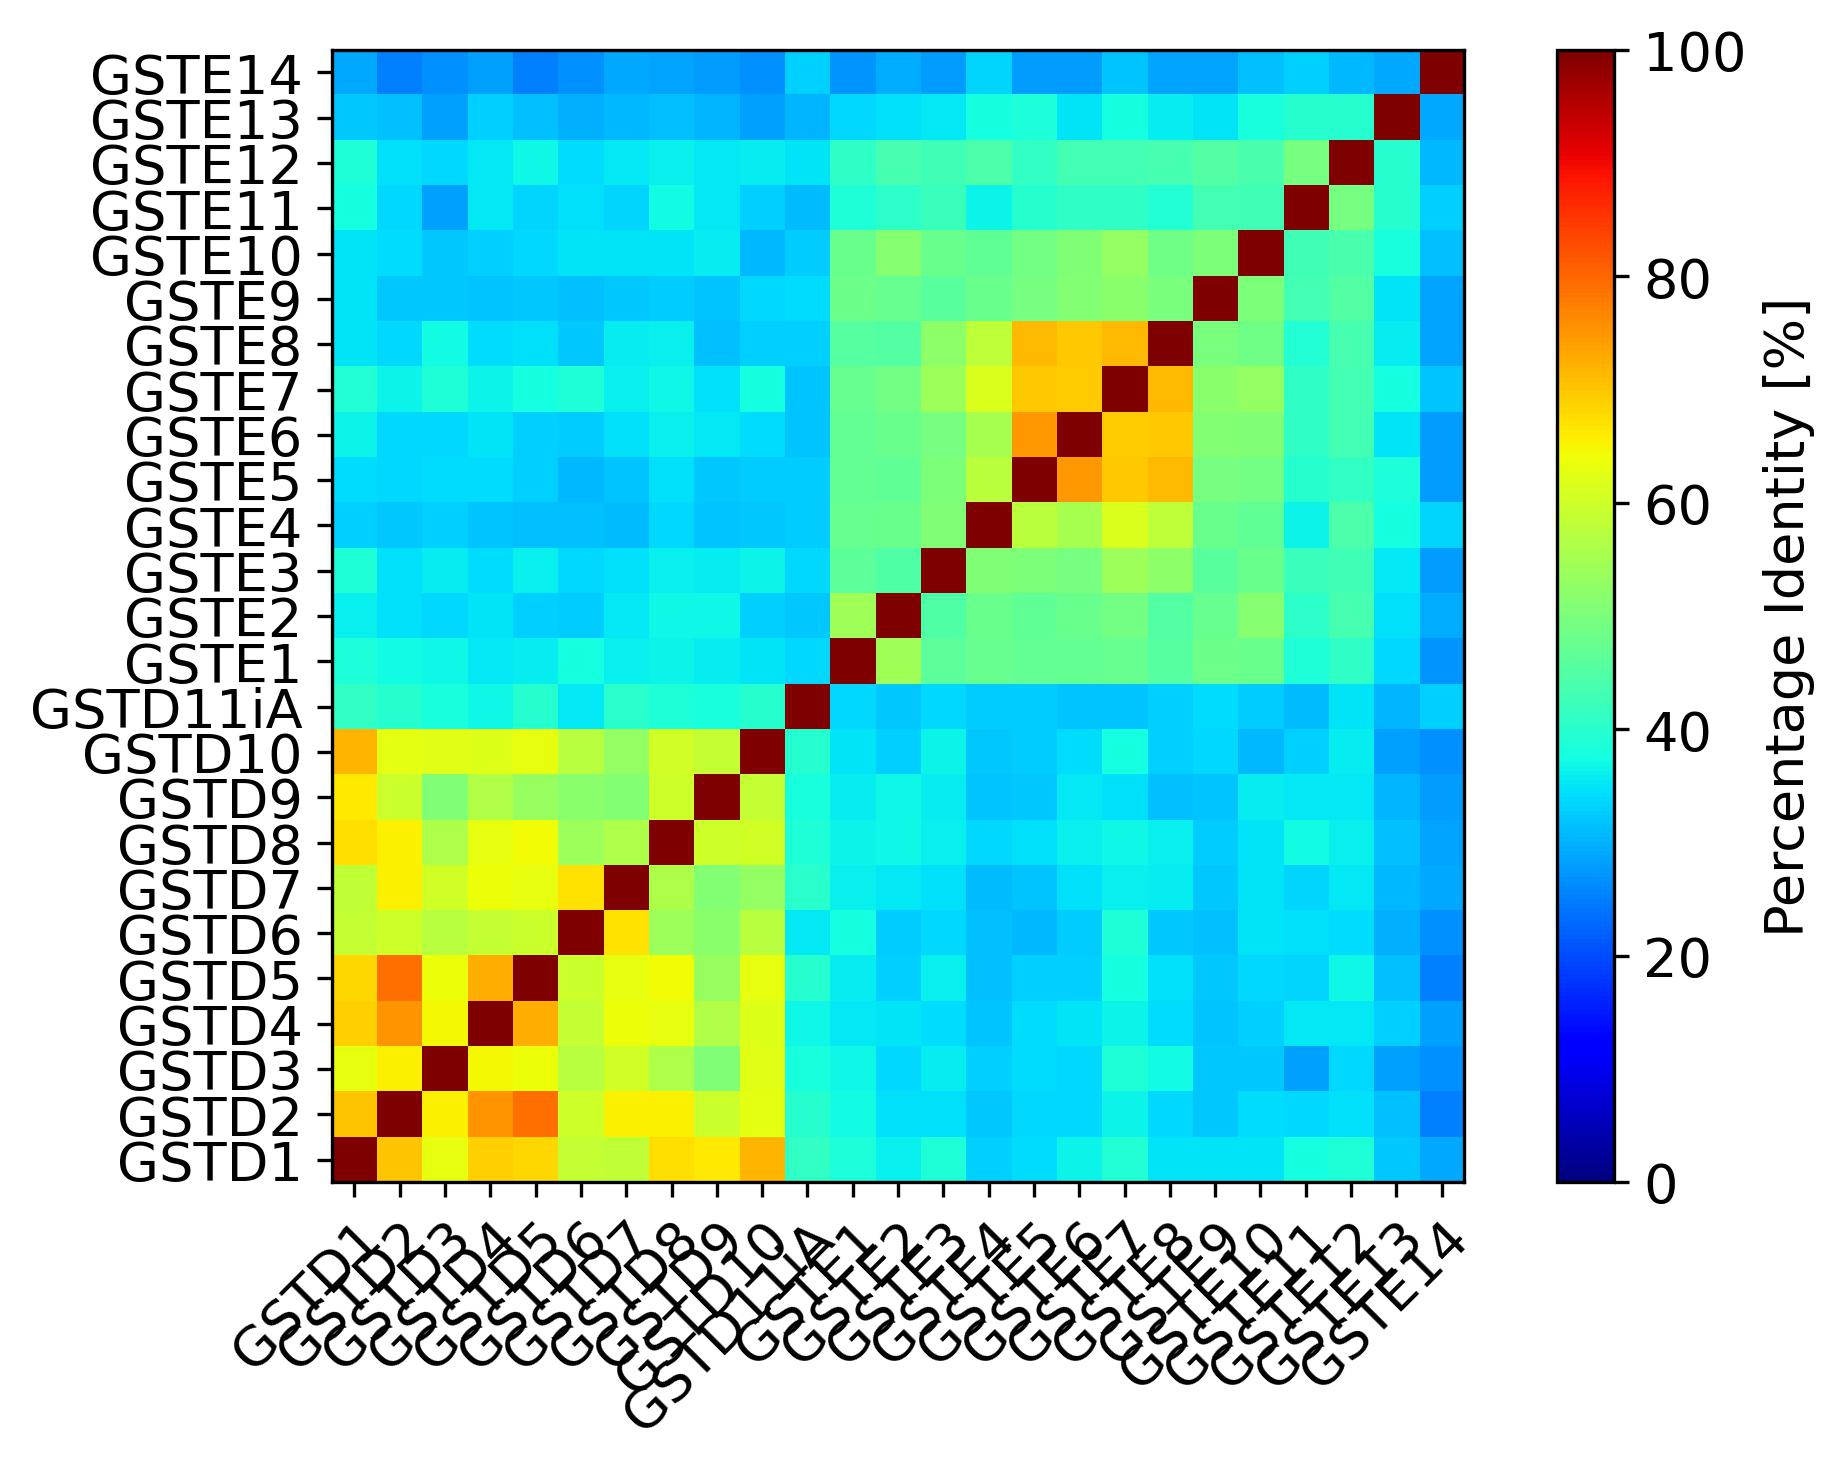
\includegraphics[height = 5cm]{figures/PercentID_matrix.jpg}
	\end{minipage}
	\begin{minipage}{.48\linewidth}
		B)\\
		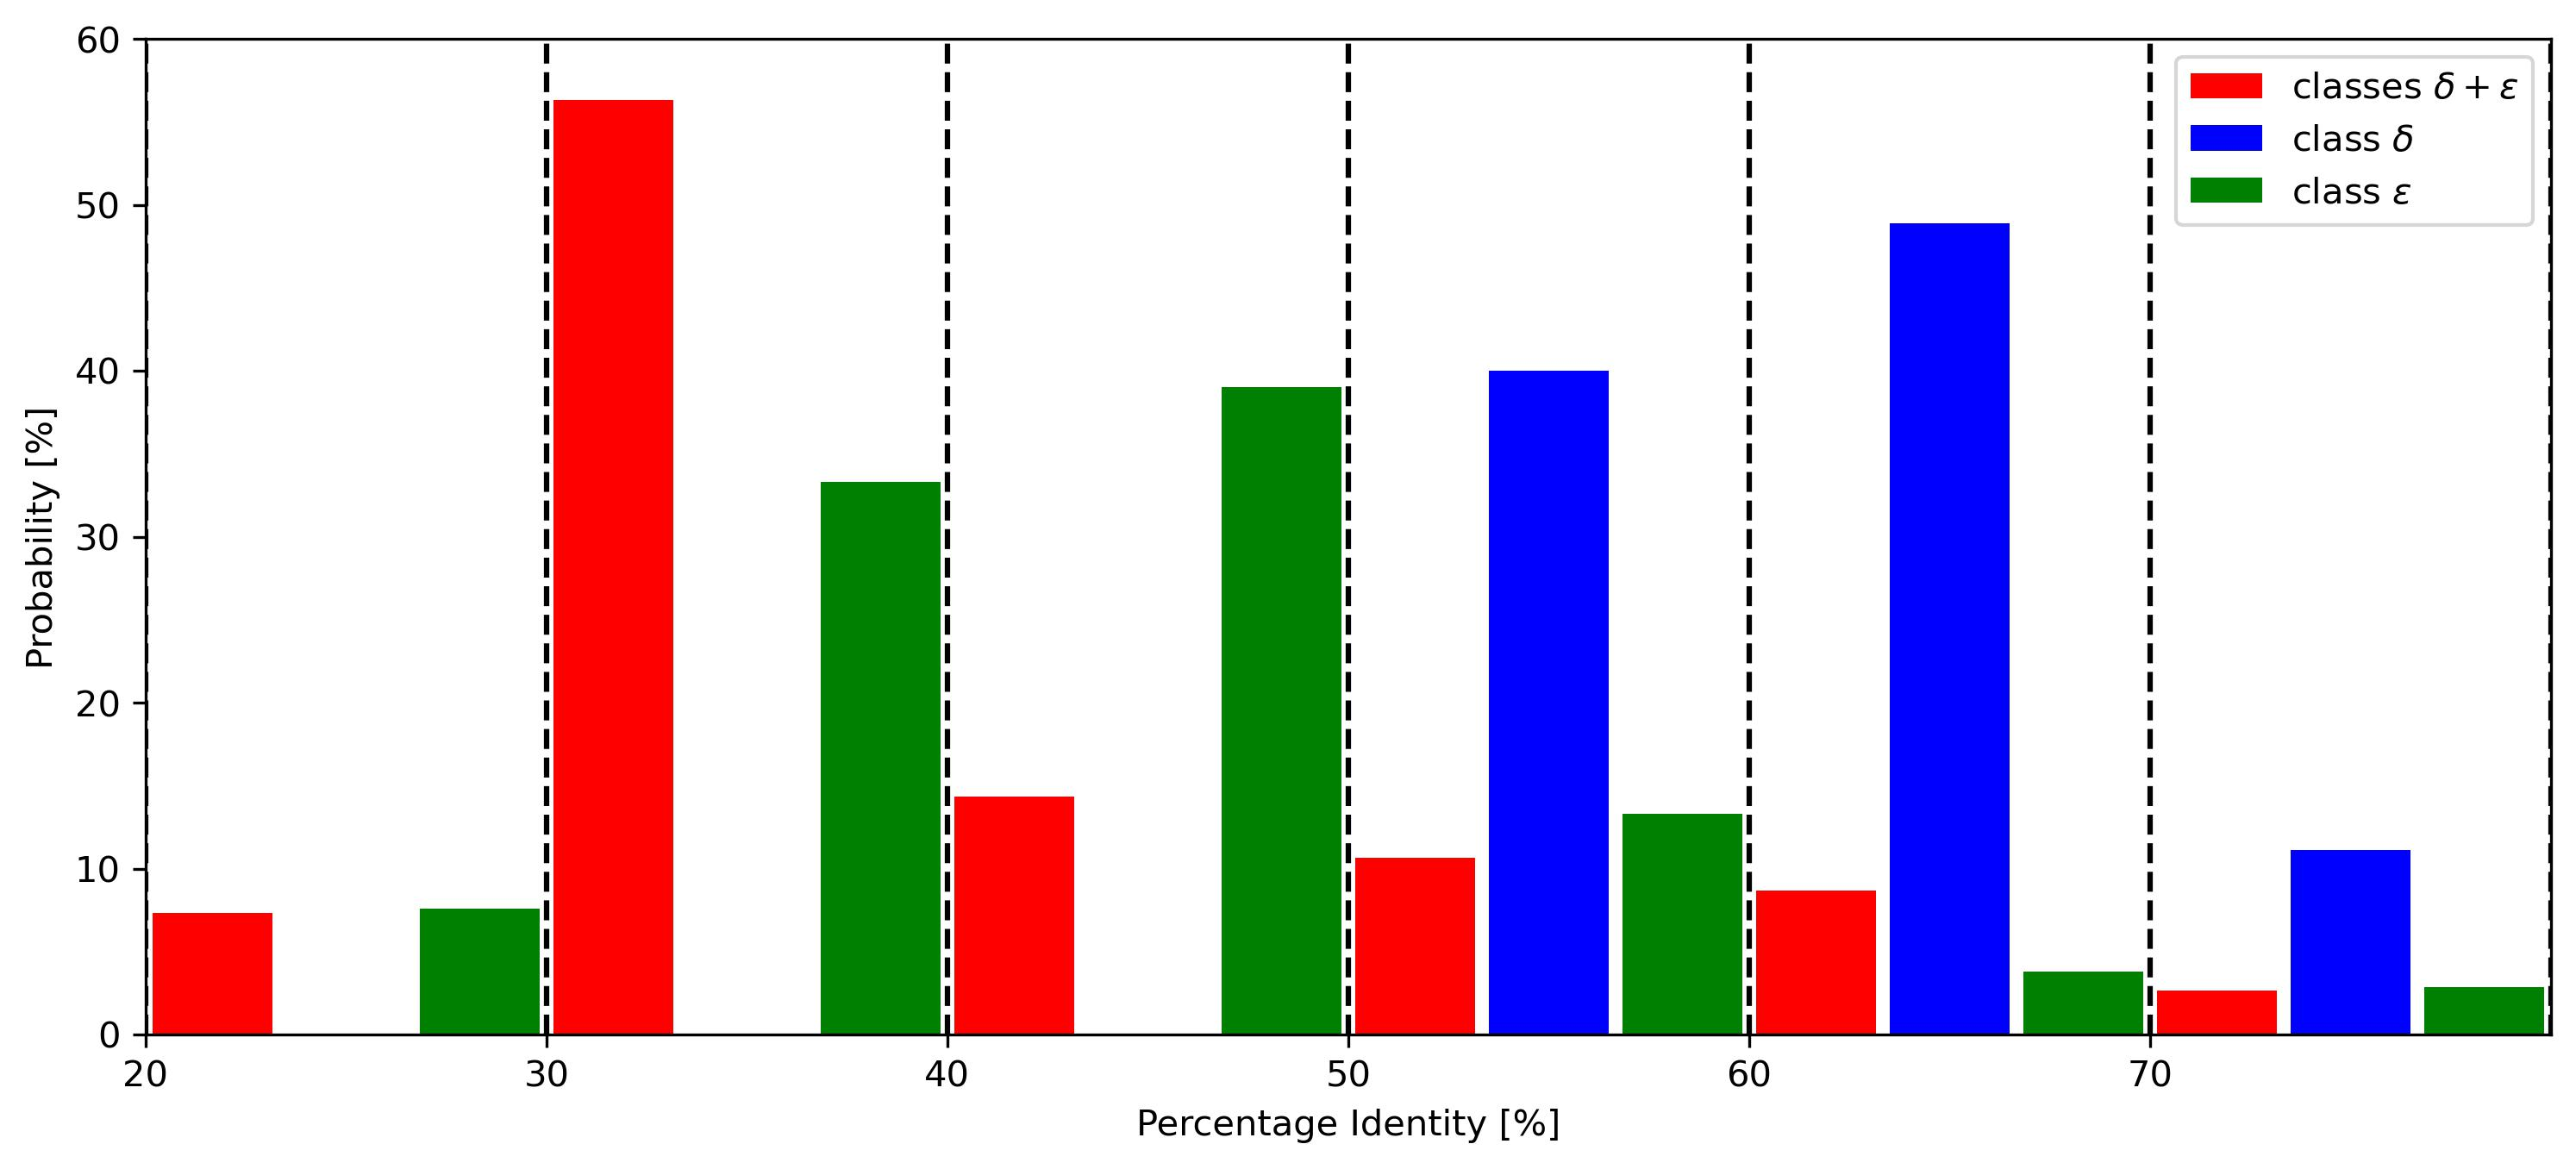
\includegraphics[height = 5cm]{figures/PercentID_proba.jpg}
	\end{minipage}
	\caption{Percent identity matrix and probability from the GST sequences}
\end{figure}

\section{Static structures predicted from AlphaFold}
\subsection{APO structures}
From the set of 25 sequences, we used AlphaFold to predict the associated 3D structure. Pairs of structures were compared using the Root Mean Squared Deviation (i.e. geometrical distances between atoms, Fig \ref{AlphaFill & GSHs} pannel A). In the associated RMSD matrix, one can identify two main clusters for class $\delta$ and $\varepsilon$. However the GSTE10 gives higher values than other $\varepsilon$ GSTs. This is due to a longer sequence in the C-terminal part with an extra $\alpha$-helix that makes the RMSD higher.

\begin{figure}
	\label{AlphaFold structures}
	\includegraphics[width = .99\linewidth]{figures/GSTs_array}
	\caption{GST's structures predicted from AlphaFold}
\end{figure}

AlphaFold does not associate any secondary structure to most of the $\varepsilon$ GSTs.

\subsection{GSH structures}
From the GSTs, we used AlphaFill to get insight in the various ligands position. In average, the predictions give 40 different Glutathione-like predictions in the structures that will be taken into account. Figure \ref{AlphaFill & GSHs} pannel B) show the predictions of AlphaFill in the case of the GSTD1. The 40 GSHs are associated to a unique monomere (chain A) but for the computations, we took into account the GSHs for the full dimeric structure.

\begin{figure}[H]
	\label{AlphaFill & GSHs}
	\begin{minipage}{.48\linewidth}
		\textbf{A}\\
		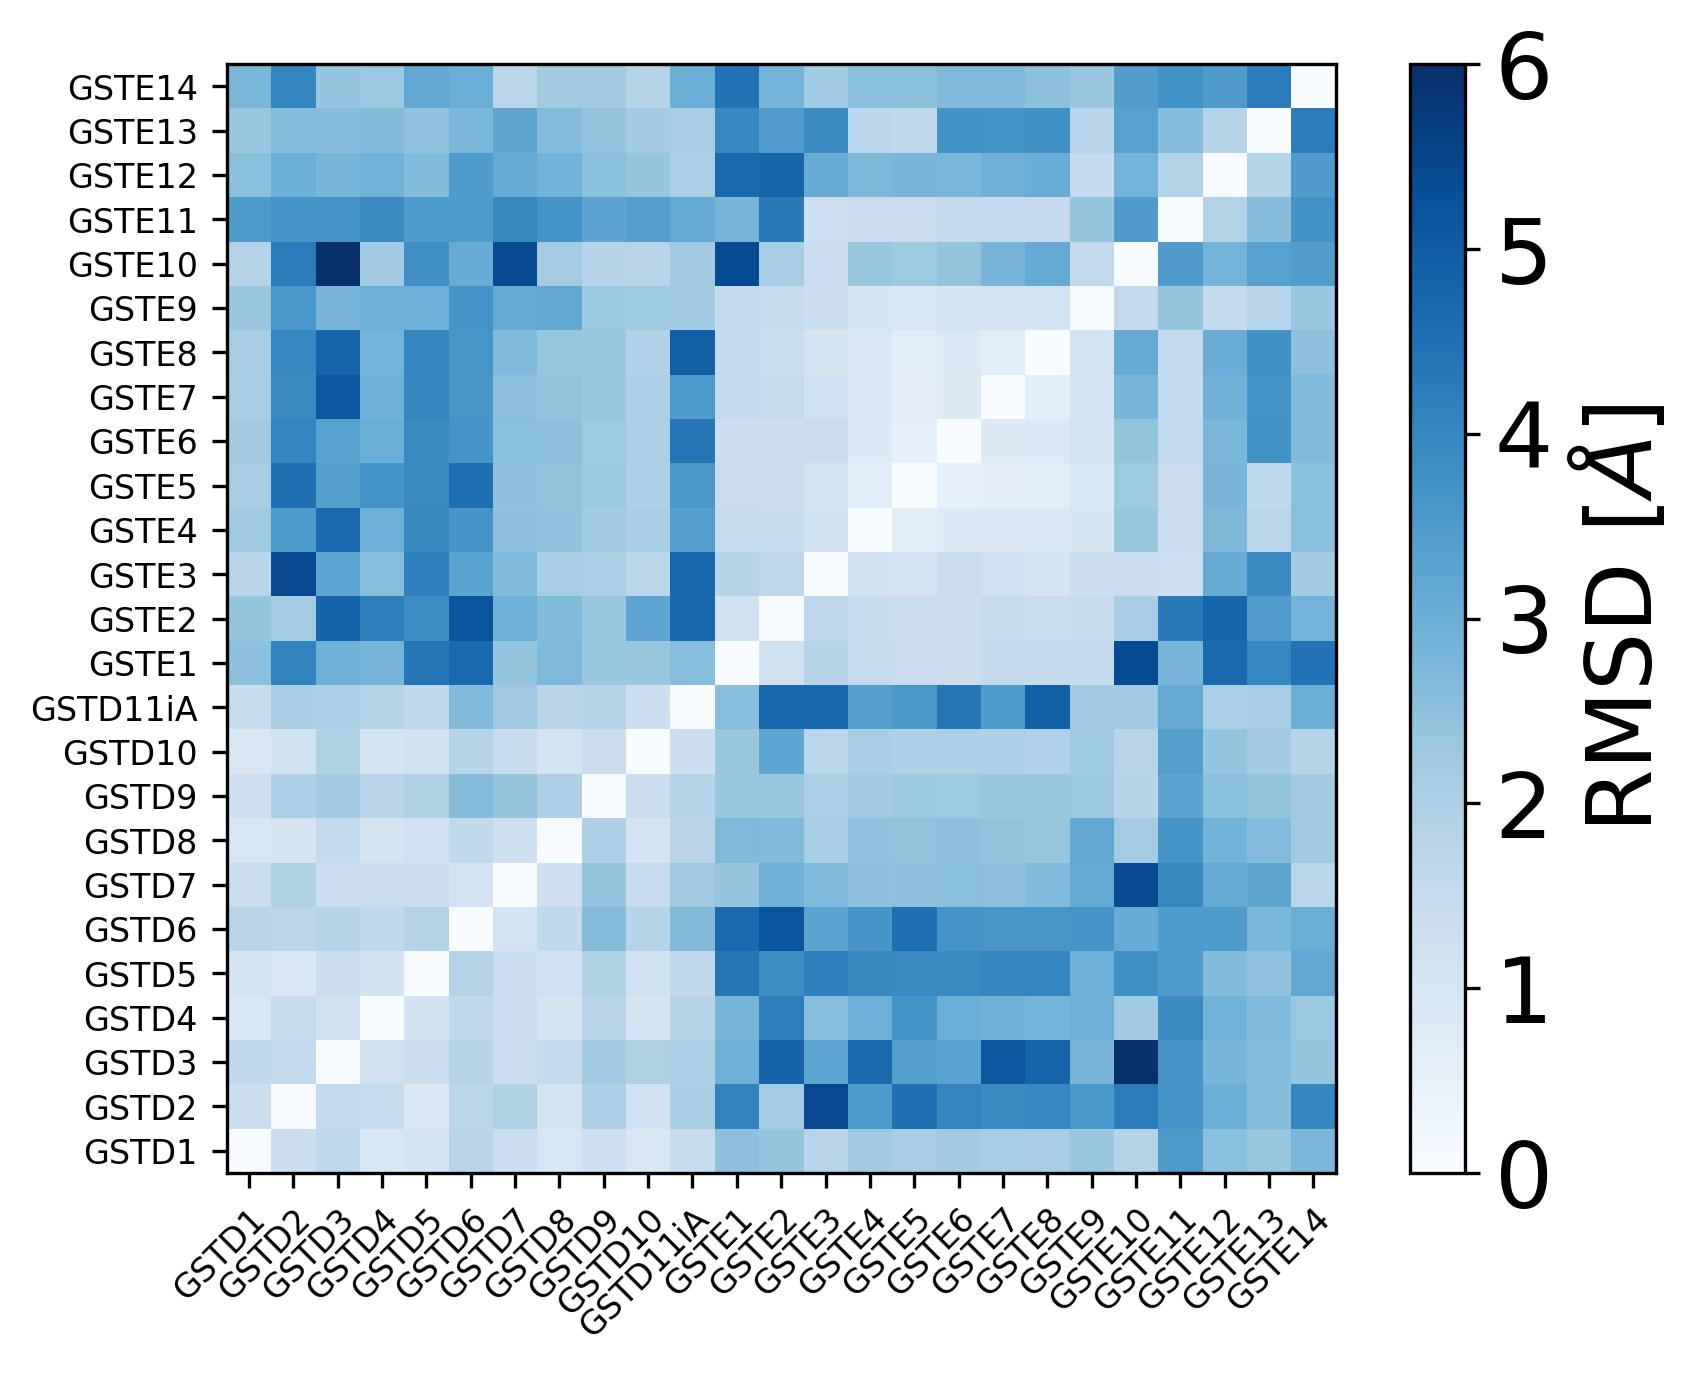
\includegraphics[height = 6cm]{figures/RMSD_matrix.jpg}
	\end{minipage}
	\begin{minipage}{.48\linewidth}
		\textbf{B}\\
		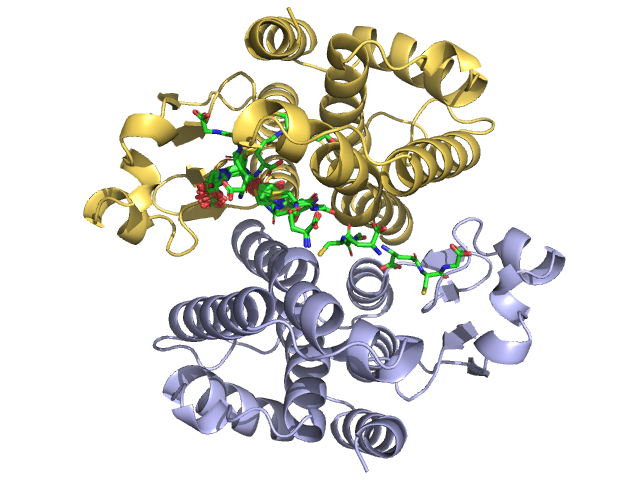
\includegraphics[height = 6cm]{figures/GSTD1_GSHs.png}
	\end{minipage}
	\caption{Geometrical comparitions between AlphaFold predicted structures \& illustration of the predictions of AlphaFill in the case of the GSTD1}
\end{figure}

\section{Conservation}

\noindent From the structures and based on distance matricies between the atoms, it is possible to look at the interface of dimerization (i.e. the residues that are involved in the monomer-monomer binding). We also used this method to determine the Binding site of the ligands. As mantioned earlier, the program AlphaFill allows to make such precisions and this gives $40$ different positions of Glutathion-like ligands in the GSTD1 (i.e. ligands that are chemically close to Glutathione), those positions are represented in the 3D structure (figure \ref{AlphaFill & GSHs} pannel B). Distances between atoms allowed us to determine from these data the residues that are involved in the protein-ligand binding as well as the dimerization of the structure. Indeed, two atoms that are closer than $3$\AA ~were considered as in contact. This information can be computed for all 25 structures and projected on the MSA matrix computed before. This gives the following representation (see Fig. \ref{MSA + AF + AFi}), where we computed the probability of a given residue to be in the binding site or in the interface of dimerization. From this information, we are able to compute the conservation of any residue in the binding site / interface of dimerization. Here, we give an illustration in the case of the residue $124$, which have a high degree of conservation among all the studied GSTs and have been identified as a part of the binding site in $\%$.

\begin{figure}[H]
	\label{BS & DI Proba}
	\center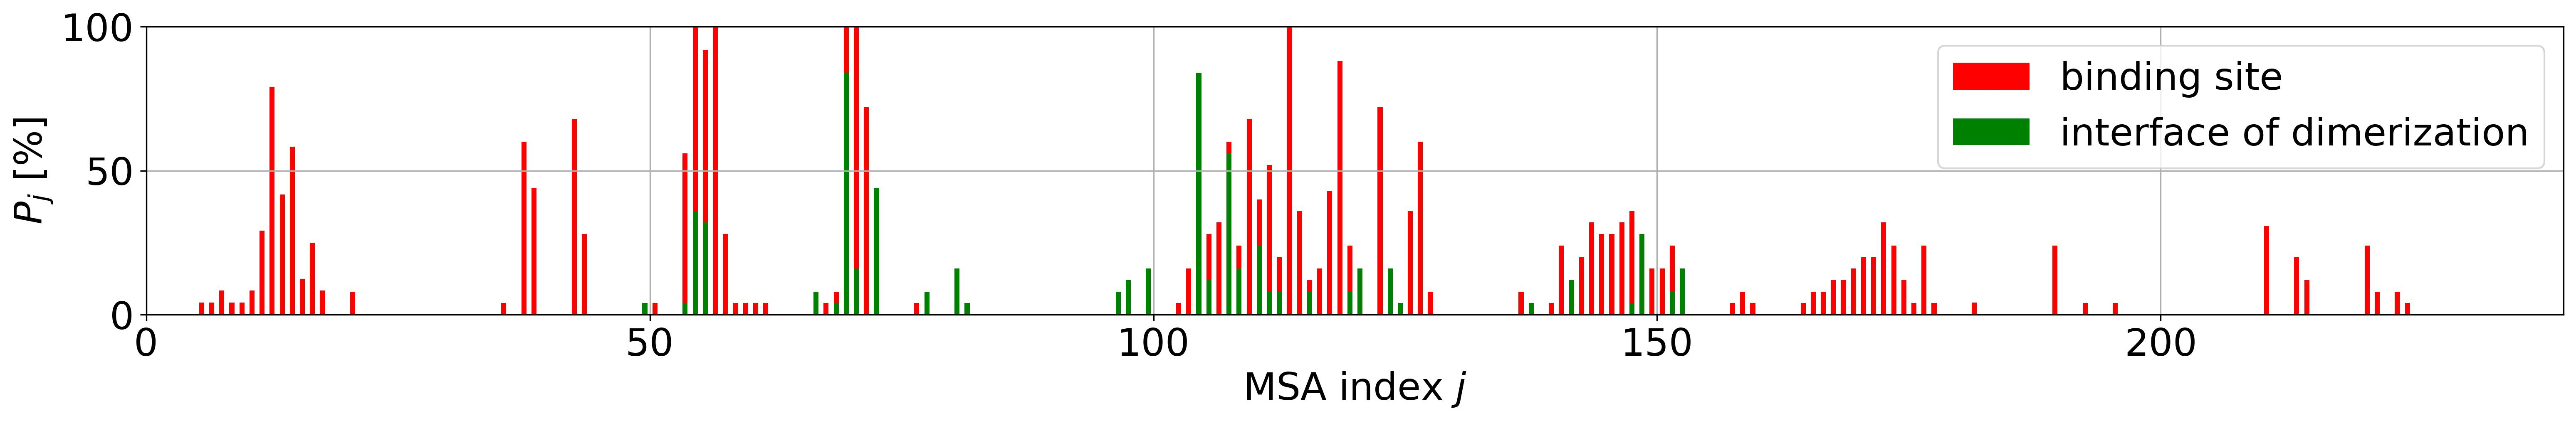
\includegraphics[width = 16cm]{figures/MSA_Proba.jpg} % BS & DI proba
	\begin{minipage}{.48\linewidth}
		\centering
		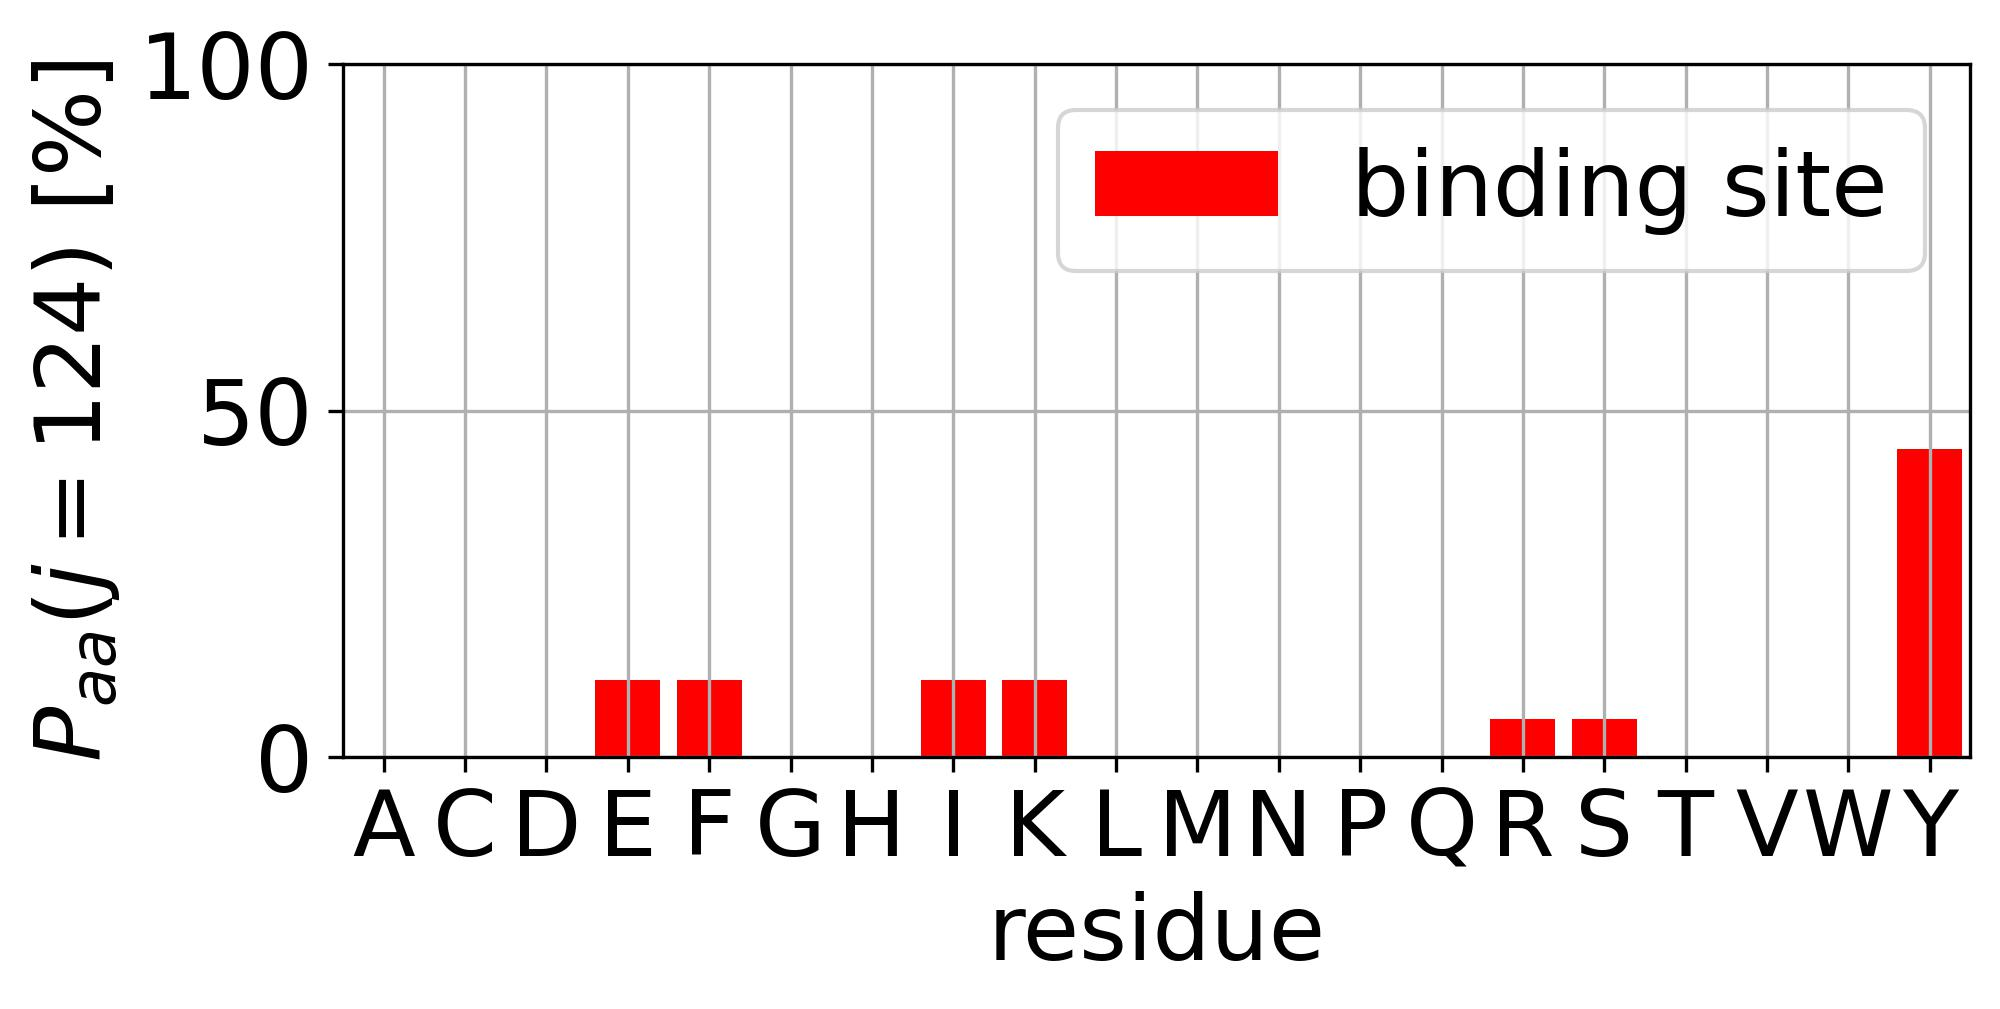
\includegraphics[width = 8cm]{figures/amino-acid_conservation_BS_j=124.jpg}
	\end{minipage}	
	\begin{minipage}{.48\linewidth}
		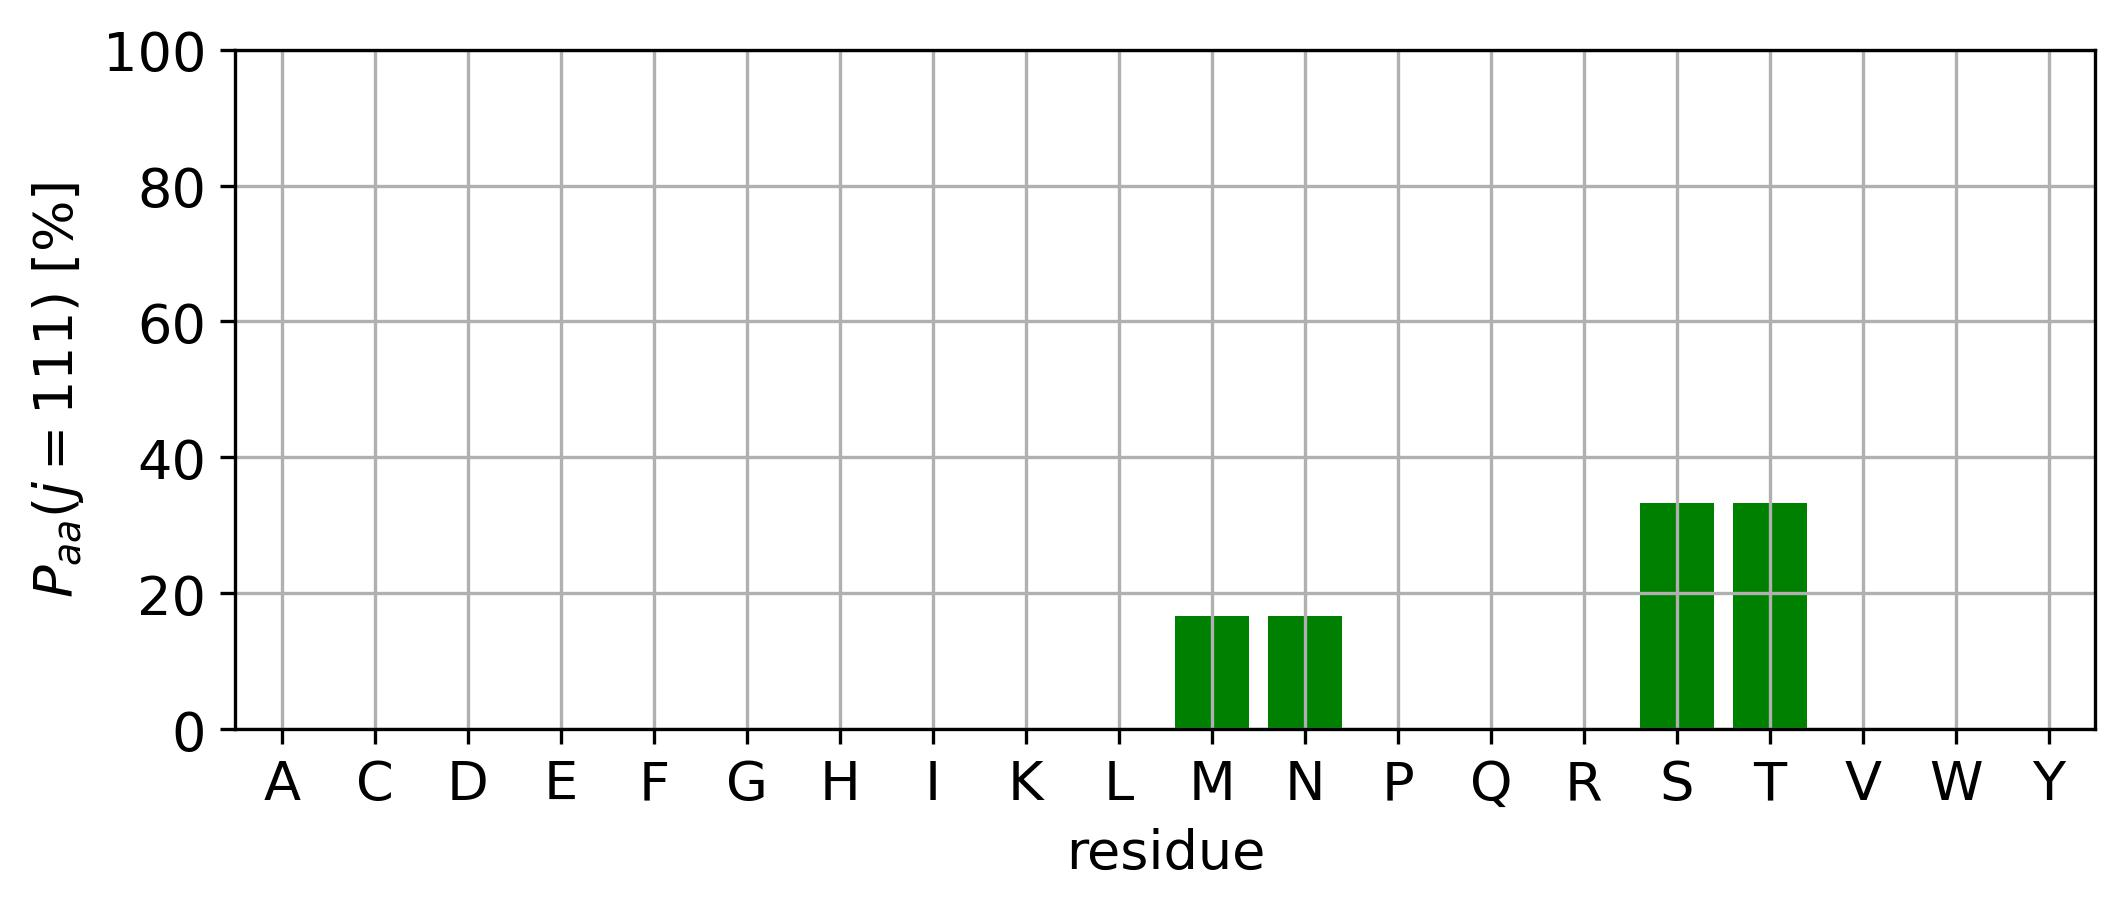
\includegraphics[width = 8cm]{figures/amino-acid_conservation_DI_j=111.jpg}
	\end{minipage}	
	\caption{Probability of a residue to be in the binding site / interface of dimerization and amino-acid conservation for the 39$^{\text{th}}$ residue of the MSA matrix that have been identified in the binding site}
\end{figure}
%In the present case, GSTs have usually Tyrosine amino-acids and looking at the MSA matrix, it seems to be especially the case for GSTs of class $\delta$ with any Tyrosine at $j = 124 ~$among the $\varepsilon$ class ! In a more precise way, it doesn't seems that in the $\varepsilon$ class the residues have any form of consevation for this particular index.
\section{Structural Dynamics from Normal Mode Analysis}
% \noindent As explained in the introduction, this present work not only cares about the informations that have been extracted from the static predictions of the AlphaFold and AlphaFill programs but also about the dynamics of the dimers. In this section we will present the next step of our methodology with the Anisotropic Network Model, starting with the parametrization.

\subsection{Local mean square fluctuations}
Figure \ref{Local MSF D1} presents the predicted Local MSF for the GSTD1 structure as well as a cartoon representation of this local fluctuation. Measured local MSF are displayed in red and predictions for the APO structure are in green. On pannel A), it apears that in $\alpha_2$ region the predicted flexibility is over estimated. On pannel B), we see that this is at the position of a kink in the secondary structure, leading to a higher flexibility. Region between $\alpha_6$ and $\alpha_7$ is also over estimated. In this case, the pearson correlation gives approximately $56\%$ of correlation.

\begin{figure}[h!]
	\label{Local MSF D1}
	\begin{minipage}{.48\linewidth}
		A)\\
		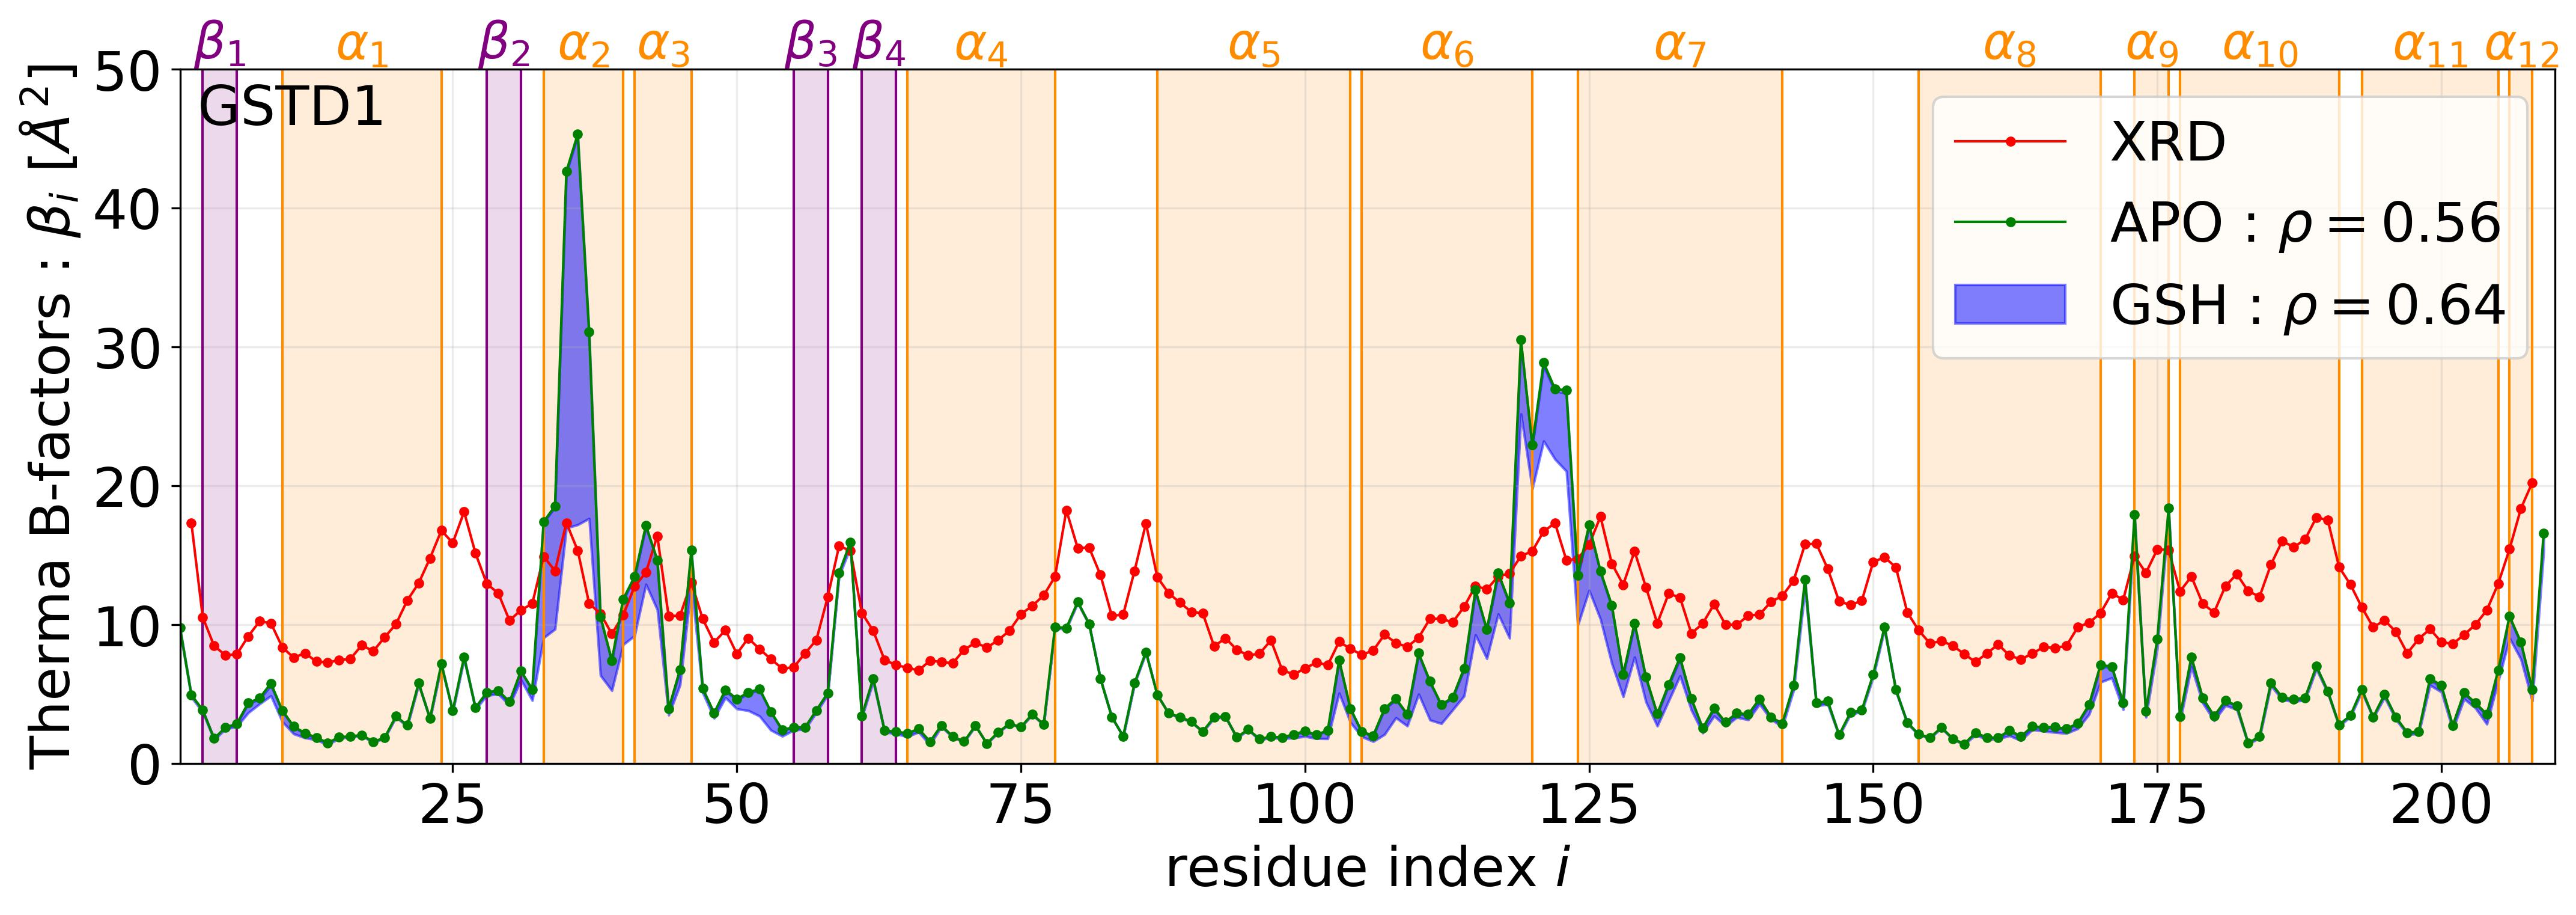
\includegraphics[width = 8cm]{figures/GSTD1+GSH_ANM-COM_Bfactors.jpg}
	\end{minipage}
	\begin{minipage}{.48\linewidth}
		B)\\
		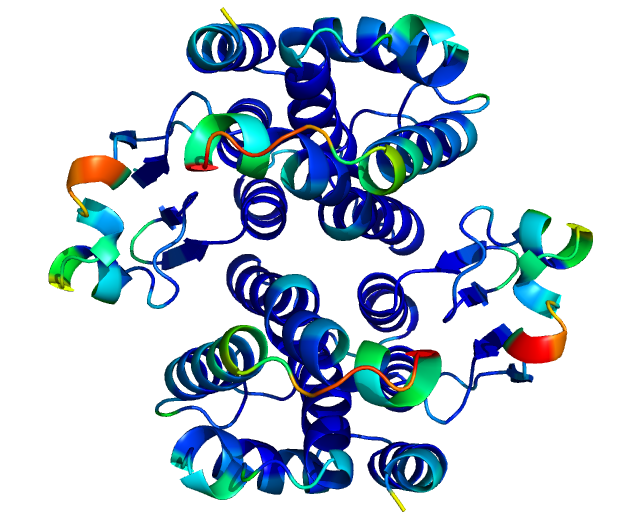
\includegraphics[height = 5cm]{figures/GSTD1_ANM-COM_Bfactors_structure.png}
	\end{minipage}
	\caption{Local mean square flucturations predicted from ANM-COM and comparisions with XRD measurments}
\end{figure}

\noindent From the 40 structures containing the ligands, we computed the range of local MSF displayed in blue. It apears that the regions that were over estimated have now a reduced flexibility with an improved pearson correlation computed from the minimum of this range. We extended the computation of the local flexibility to the ensemble of structure and projected the flexibility on the MSA matrix. 

\begin{figure}[h!]
	\label{ANM-COM + MSA}
	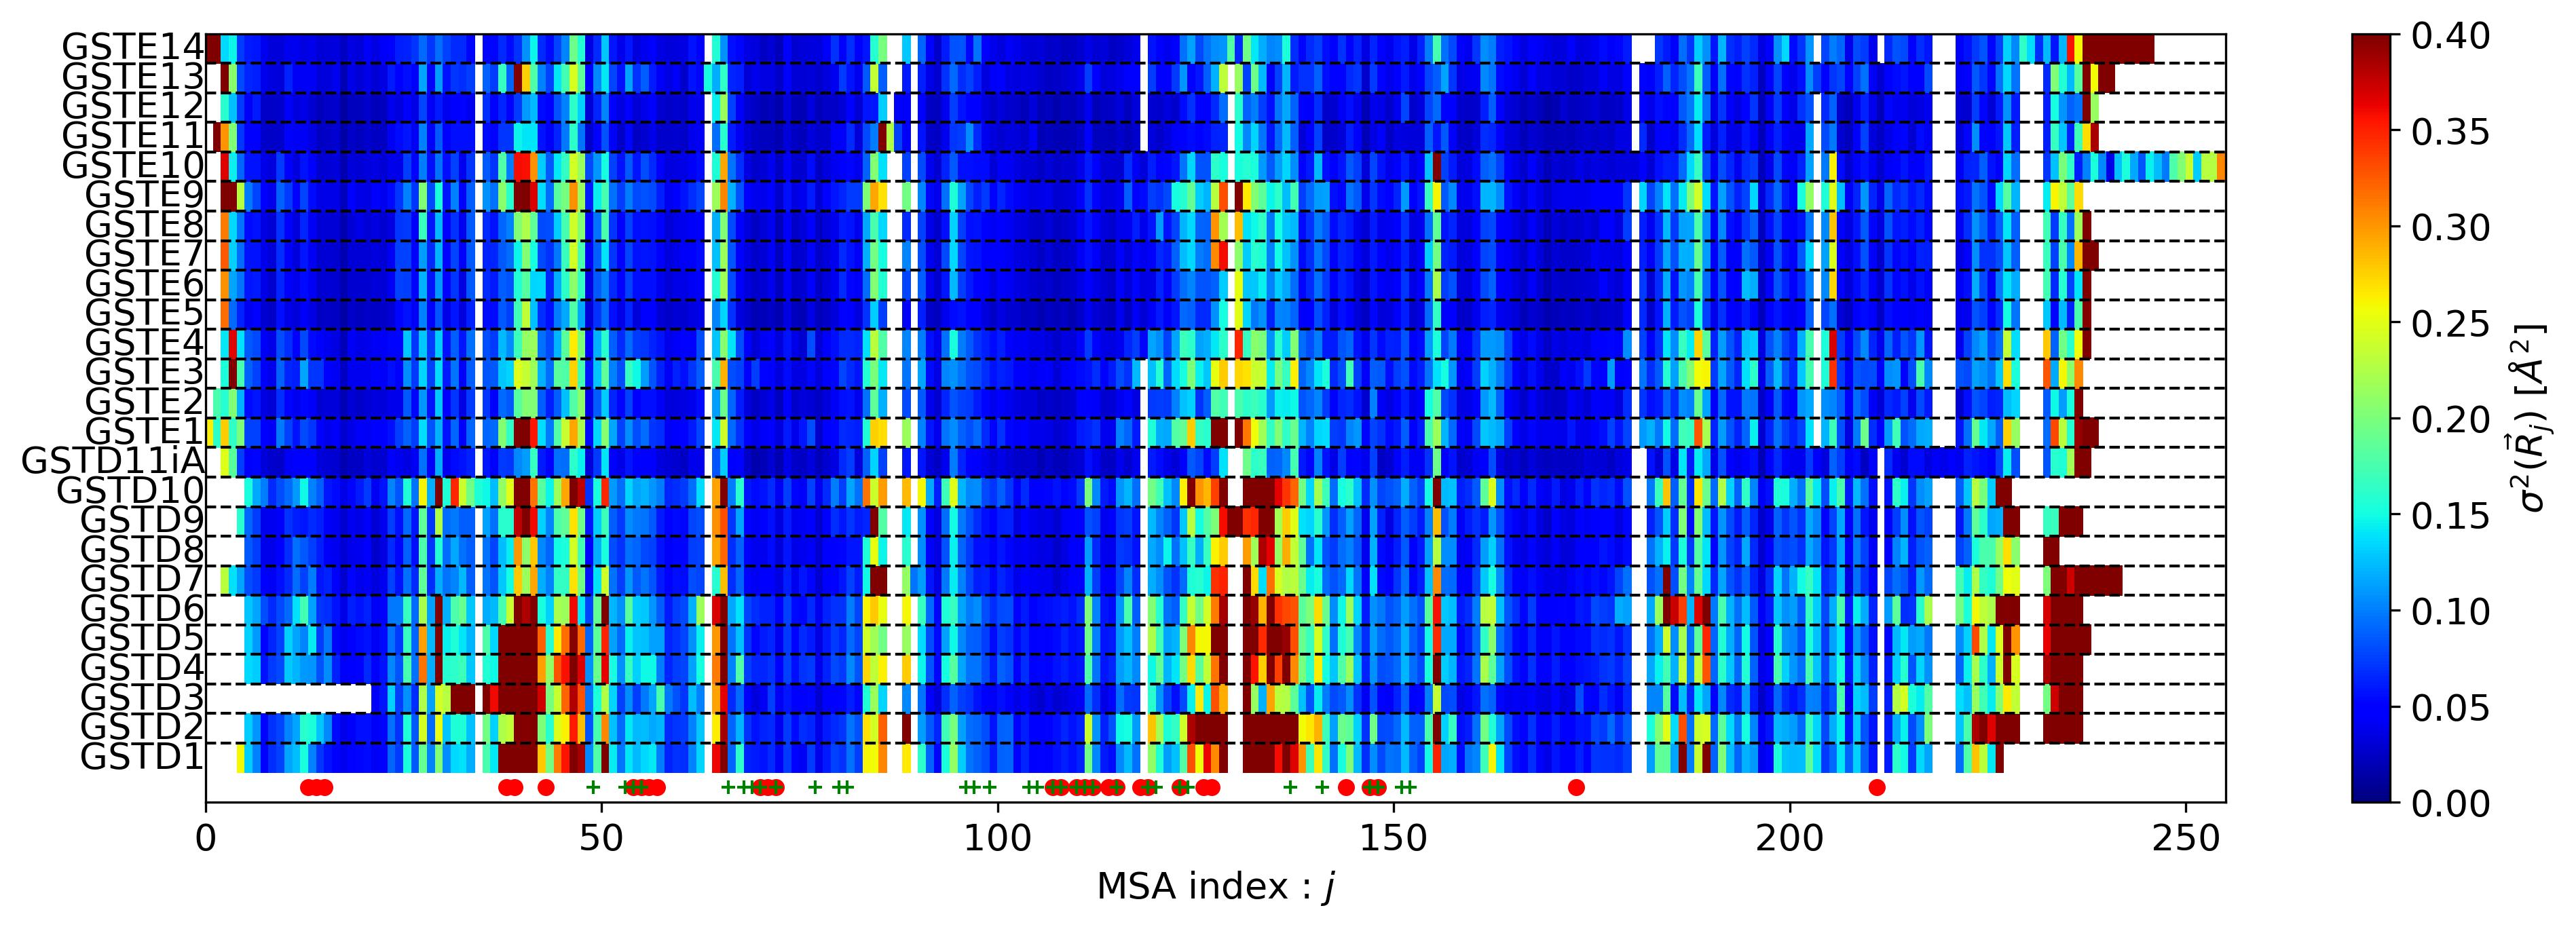
\includegraphics[width = .99\linewidth]{figures/ANM-COM+MSA_APO_MSF.jpg}
	\caption{Local flexibility computed from APO structures and projected on MSA matrix}
\end{figure}

\noindent From this map, we can identify regions of conserved high flexibility. First we identify that the terminal parts are much more flexible than the rest of the structures. Second we identify regions of conserved high flexibility between MSA indicies $40-42$. We also identify the $30^{\text{th}}$ residue and the residues $129-135$ to be highly flexible which is very specific to the $\delta$ class. Taking into account the influences of the GSHs, we computed the local rigidity induced by the presence of the ligands in the structure. This is achieved by computation of the MSFs for each GSH structure and compute $(\text{MSF}_{\text{APO}} - \text{MSF}_{\text{GSH}}) / \text{MSF}_{\text{APO}}$.

\begin{figure}[h!]
	\label{Local rigidity GSHs}
	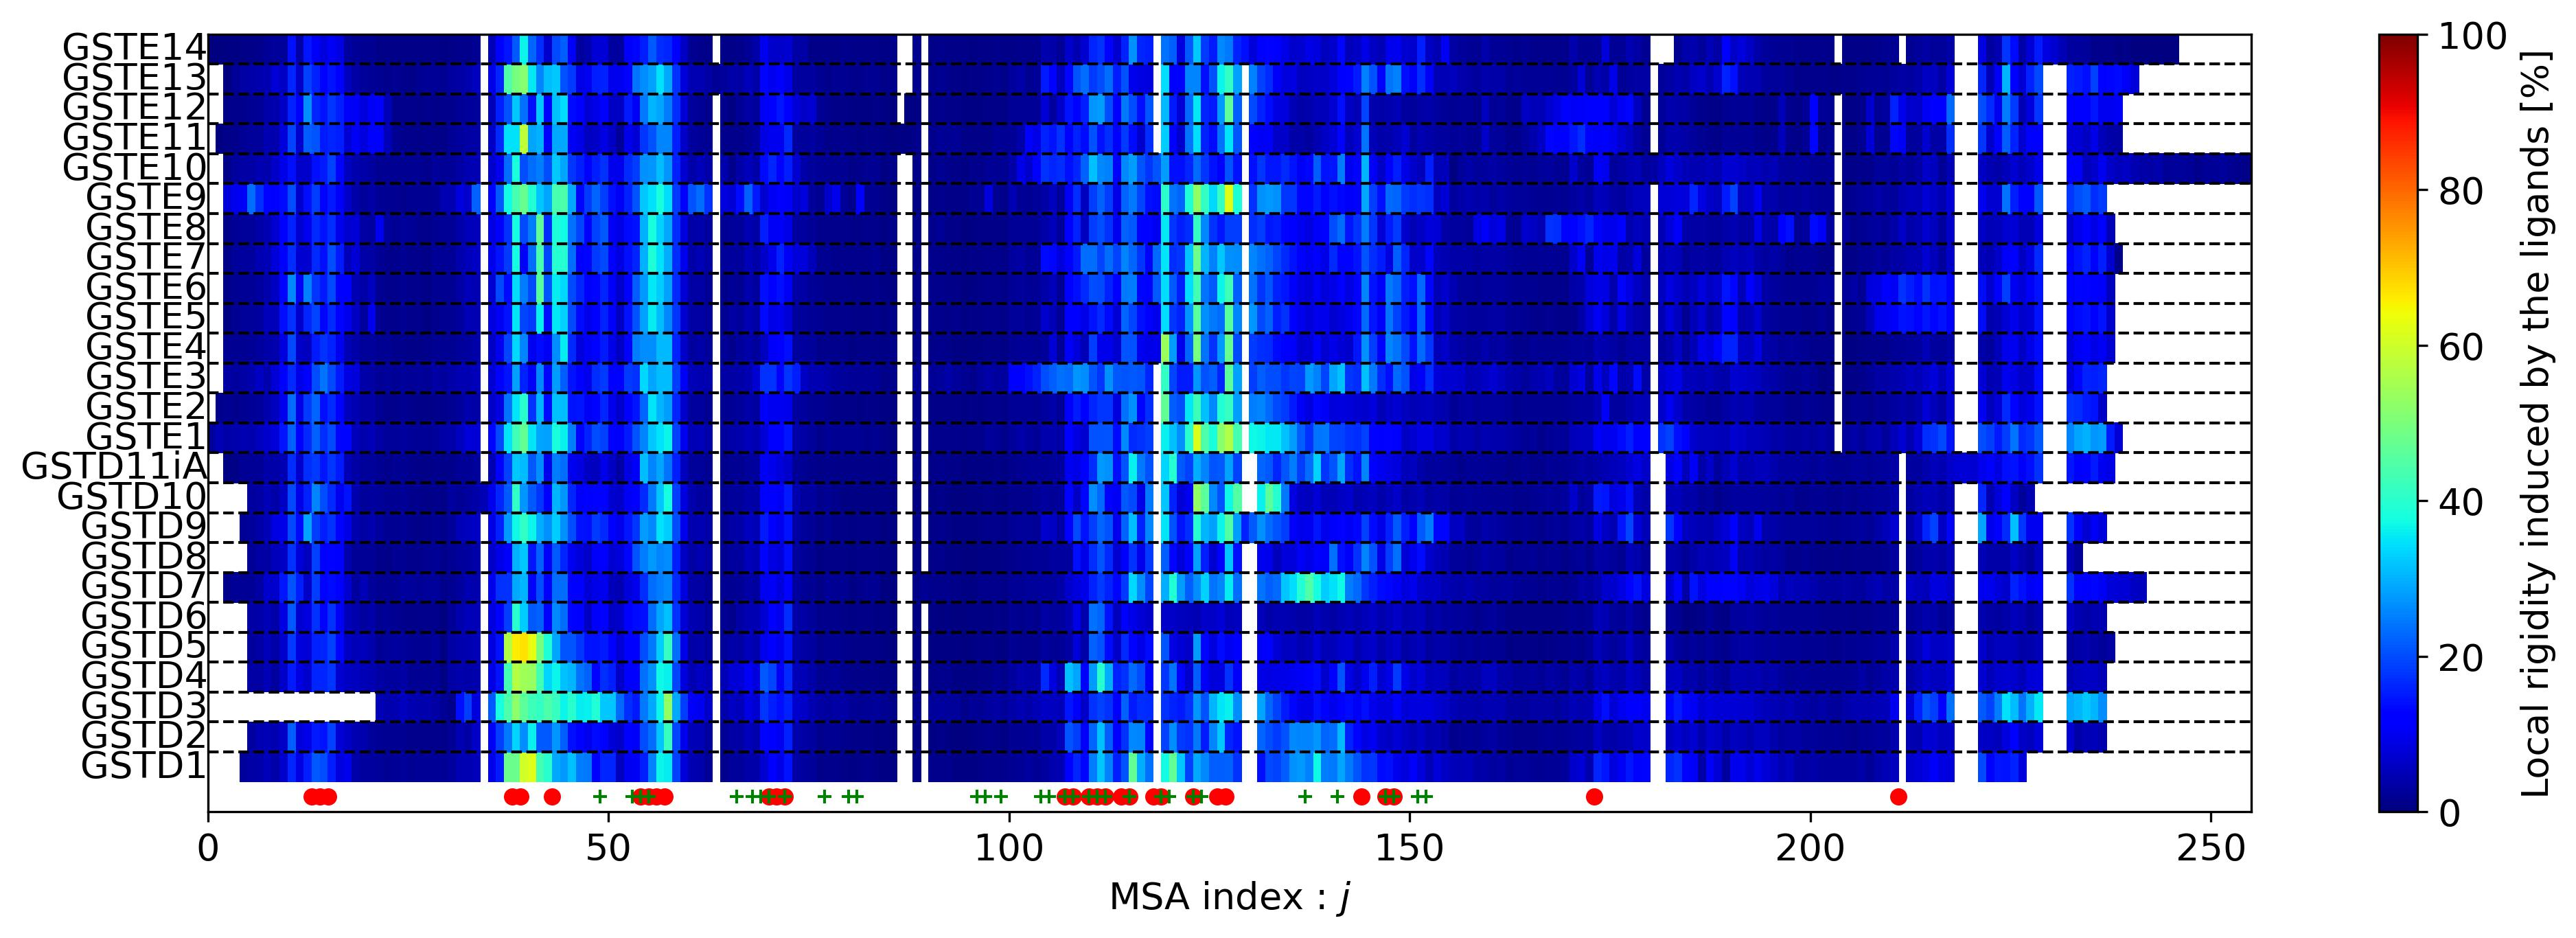
\includegraphics[width = 16cm]{figures/ANM-COM+MSA_GSHs_influcene_MSF.jpg}
	\caption{Local rigidity induced by the GSHs predicted from AlphaFill}
\end{figure}


\subsection{Non-local mean square fluctuations}

Figure \ref{Non-local MSF GSTD1} represents the non-local mean square fluctuations computed from the equation (\ref{}) and from the GSTD1 structure. In the associated matrix, we identifie lines of high non-local MSF. In particular, one can identify intersections between two lines. This allows to identify key pairs of high non-local MSF. In GSTD1, we identified the pairs of amino-acid $30;122$ ... 
\begin{figure}
	\label{Non-local MSF GSTD1}
	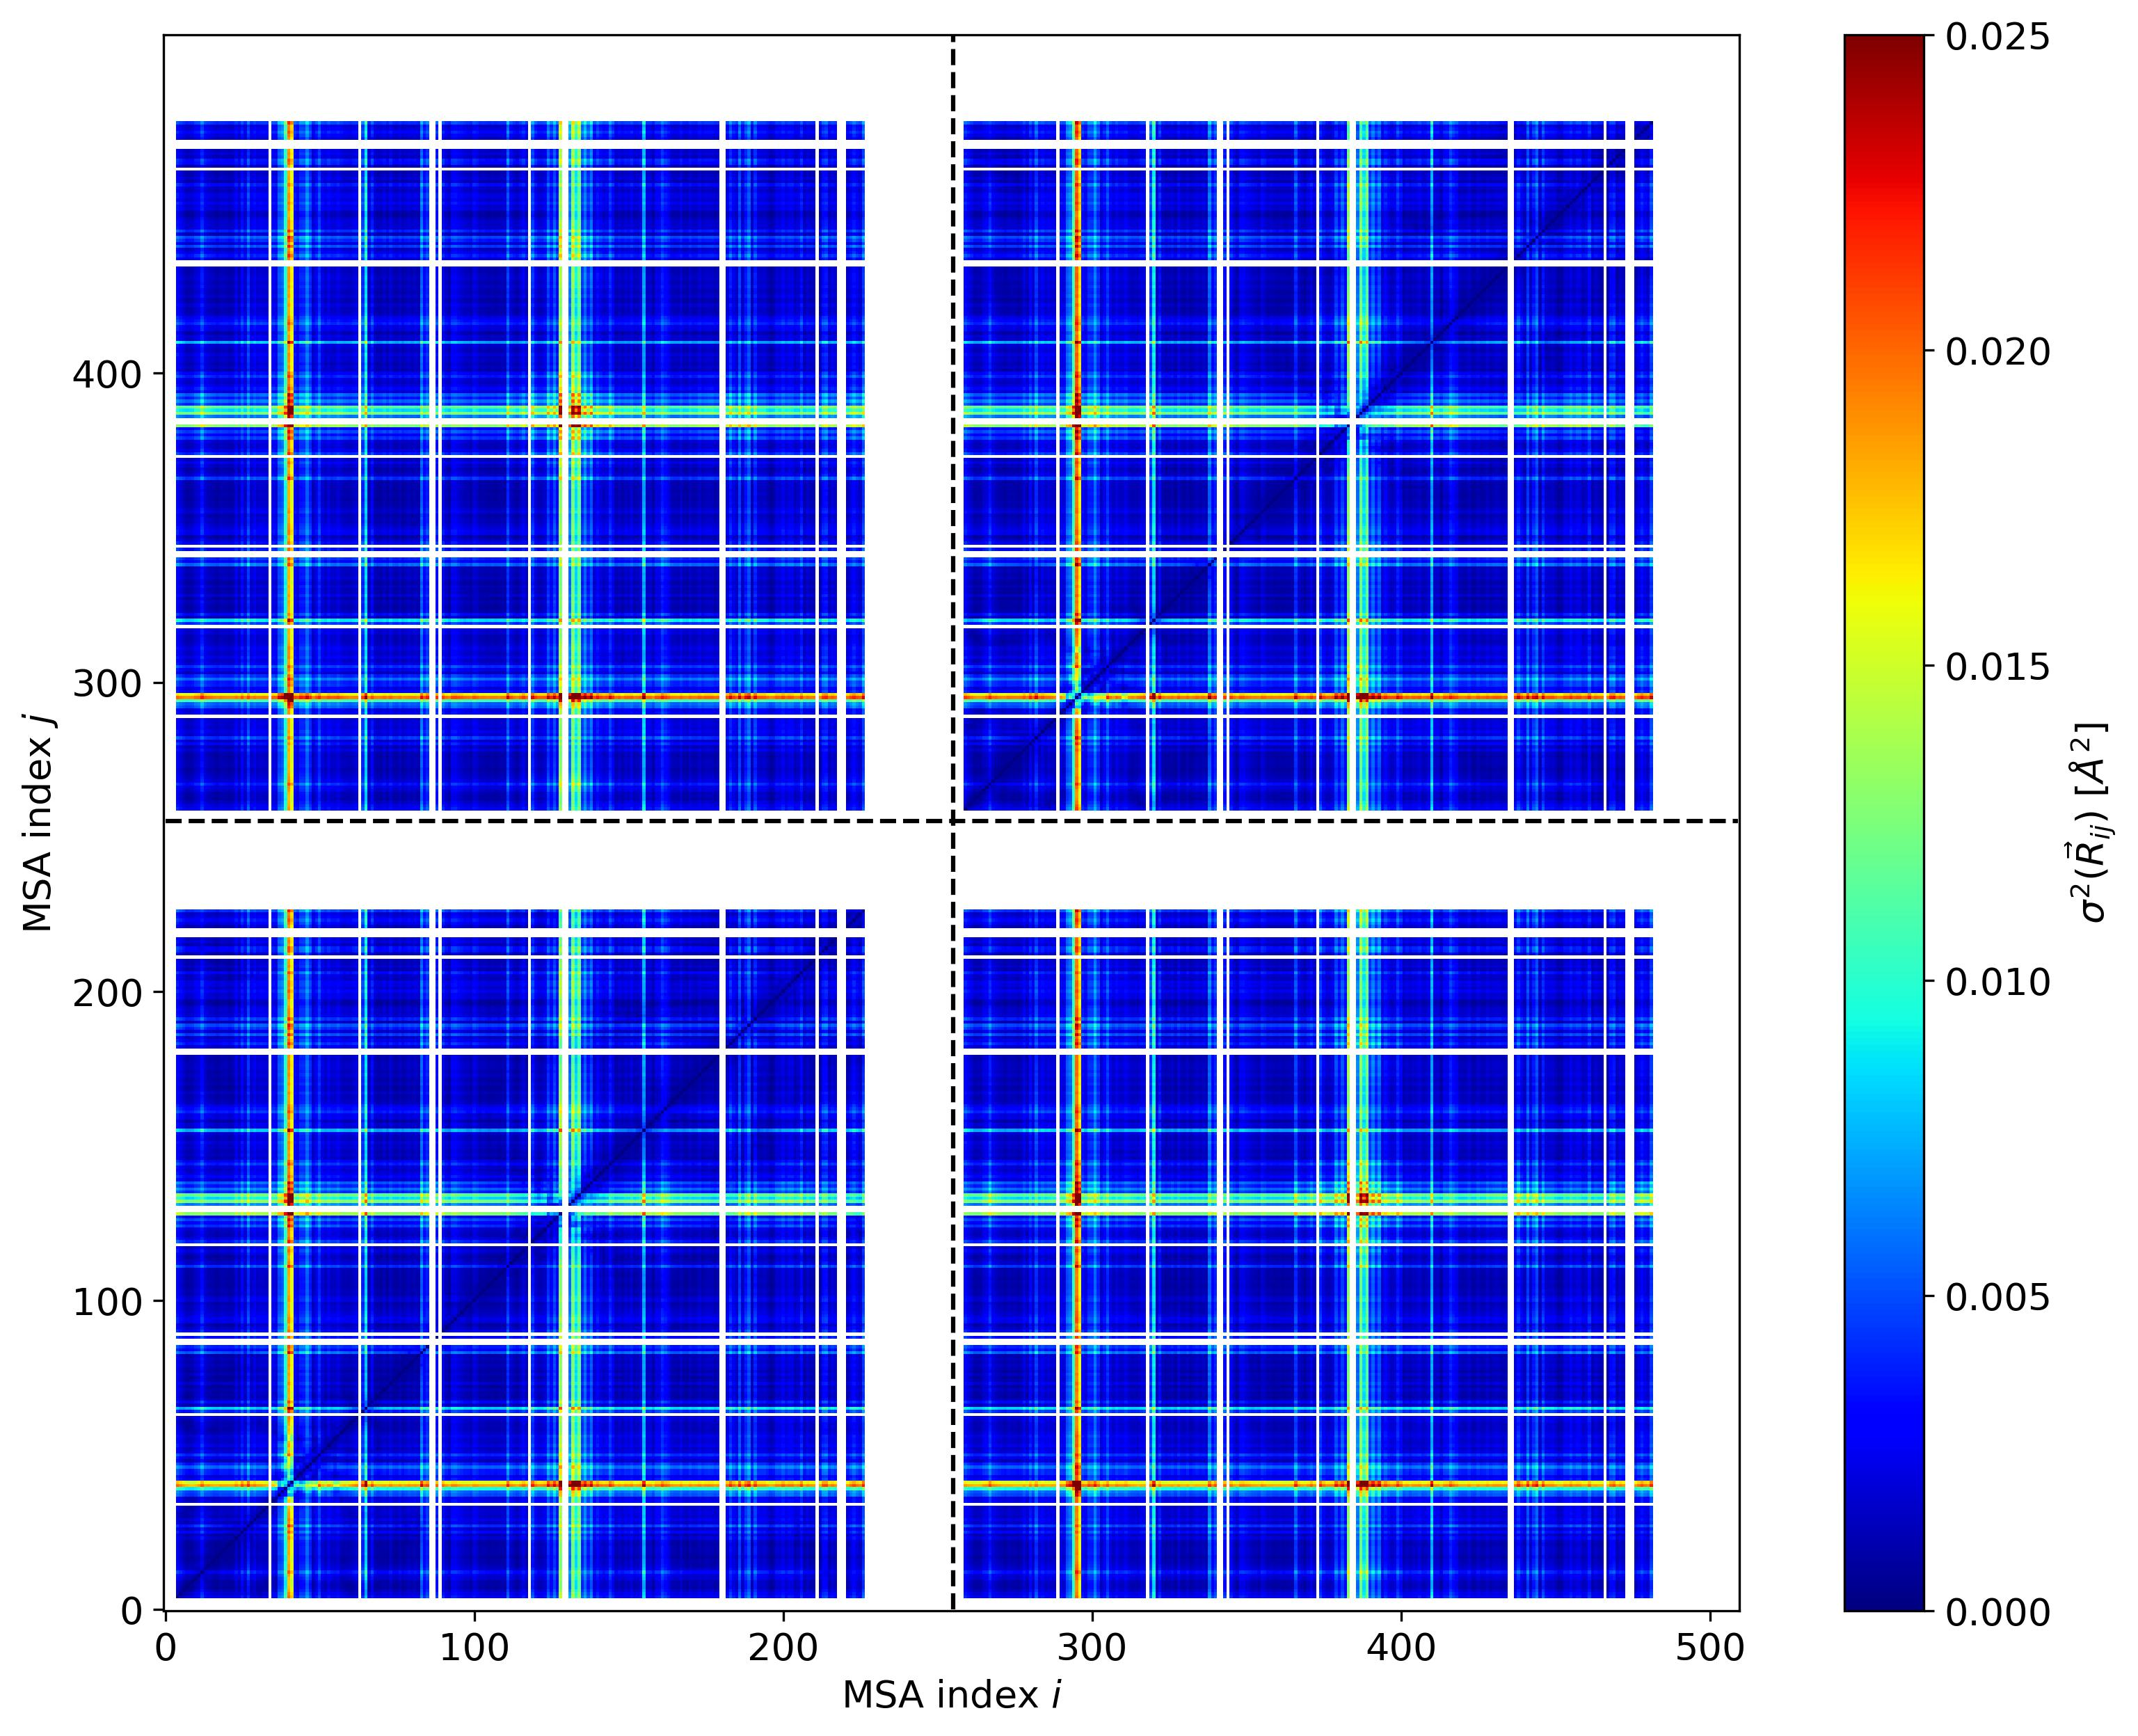
\includegraphics[width = 8cm]{figures/ANM-COM+MSA_GSTD1_APO_non-local_MSF}
	\caption{Non-local MSF matrix computed for the GSTD1 structure}
\end{figure}

\section{Identification of conserved key residues}

From the computed local and non-local thermal MSF, we identified regions of high flexibility. From the local MSF, a value above $0.25$\AA$^2$ is associated to a high flexibility. For non-local MSF, a pair with a value above $0.025$\AA$^2$ is also considered as high flexible. We identified indicies that corresponds to these criteria and checked their amino-acid conservation among the 25 associated sequences. We did consider a high conservation when one of the amino-acid is conserved within more than $70\%$. Medium conservation corresponds to a peak conservation between $30$ and $70\%$ and low conservation correspond to a maximum bellow $30\%$.

\begin{table}[h!]
	\begin{tabular}{cp{4cm}p{5cm}p{4.5cm}}
		\hline
		\hline
		& High conservation & Medium conservation & Low conservation \\
		\hline
		\multirow{2}{*}{Local MSF} & •   $3$ & •  $30$ & • $33$ \\
		                           & • $190$ & •  $32$ & • $36$ \\
		                           &         & •  $34$ & • $40$ \\
		                           &         & •  $41$ & • $129$ \\
		                           &         & •  $42$ & • $132$ \\
		                           &         & •  $85$ & • $135$ \\
		                           &         & • $130$ & • $185$ \\
		                           &         & • $131$ & • $233$ \\
		                           &         & • $133$ & • $235$ \\
		                           &         & • $134$ & • $236$ \\
		                           &         & • $156$ & • $237$ \\
		                           &         & • $228$\\
		                           &         & • $229$\\
		\hline
		\multirow{2}{*}{Non-local MSF} & • resi & • resi & • resi \\
		                               & • resi & • resi & • resi \\
		\hline
		\hline
	\end{tabular}
	\caption{Identification of conserved key residues}
	\label{Final table}
\end{table}
